% Chapter 3
%----------------------------------------------------------------------------------------
\chapter{Estado del Arte} % Main chapter title
\label{Chapter3} % For referencing the chapter elsewhere, use \ref{Chapter3} 
\begin{onehalfspacing}

Este capítulo presenta las pruebas que han hecho diferentes estudios y sus resultados. A pesar de que el detectar si una persona es veraz o falsa en sus declaraciones ha sido una investigación bastante estudiada y antigua. Siguen realizando diferentes estudios y metodologías para encontrar los verdaderos rasgos que dan indicio a una verdad y a una mentira, esto con el fin de poder generalizar la tarea de clasificar verdades o mentiras.\\


David Raskin y Gunter Kohnken, especialistas en detección de mentiras, creen que detectar mentiras a través de pistas no verbales es una metodología en la que la gente no puede confiar. Detectar mentiras a través del lenguaje no verbal tiene una exactitud (porcentaje de respuestas correctas) entre el 45 y 60\%. Las personas tienen una exactitud para detectar verdades del 67\% y 44\% para detectar mentiras \cite{Vrij2000DetectingBehavior,Bond2006AccuracyJudgments}.\\

Vrij en el año 2000 \cite{Vrij2000DetectingBehavior} examinó en su trabajo la hipótesis de que a través de un análisis sistemático del comportamiento no verbal podía ser capaz de detectar mentiras y verdades en un individuo. Analizaron el lenguaje no verbal a través de dos personas que observaron y anotaron el comportamiento de videos en donde aparecían varias personas mintiendo y diciendo verdades, analizando las veces en el cual una persona desvía la mirada, sonríe, mueve los pies, mueve los dedos, etc. Obtuvieron un 78\% de exactitud en la clasificación de mentiras y verdades, mientras que un grupo de estudiantes que intentaron detectar mentiras con el mismo conjunto de datos obtuvo un accuracy del 53\%. \\ 


\begin{table}[h!]
\centering
    \begin{tabular}{|c|c|c|}
        \hline 
        feature Set & DT & RF\tabularnewline
        \hline 
        \hline 
        Unigrams & 60.33\% & 56.19\%\tabularnewline
        Bigrams & 52.71\% & 51.20\%\tabularnewline
        Facial displays & 70.24\% & 76.03\%\tabularnewline
        Hand gestures & 61.98\% & 62.80\%\tabularnewline
        Uni + Facial displays & 66.94\% & 57.02\%\tabularnewline
        \hline 
        All verbal & 60.33\% & 50.41\%\tabularnewline
        All non-verbal & 68.59\% & 73.55\%\tabularnewline
        \hline 
        All features & 75.20\% & 50.41\%\tabularnewline
        \hline 
    \end{tabular}%
	\caption{Resultados del trabajo de Verónica en el 2015}
	\label{tab:Fig_Veronica2015}
\end{table}

\begin{table}[h!]
\centering
    \begin{tabular}{|c|c|c|c|c|}
        \cline{2-5} \cline{3-5} \cline{4-5} \cline{5-5} 
        \multicolumn{1}{c|}{} & Text & Audio & Silent video & Full video\tabularnewline
        \hline 
        A1 & 54.55\% & 51.24\% & 45.30\% & 56.20\%\tabularnewline
        \hline 
        A2 & 47.93\% & 55.37\% & 46.28\% & 53.72\%\tabularnewline
        \hline 
        A2 & 50.41\% & 59.50\% & 47.93\% & 59.50\%\tabularnewline
        \hline 
        Sys & 60.33\% & NA & 68.59\% & 75.20\%\tabularnewline
        \hline 
    \end{tabular}%
	\caption{Resultados obtenidos de tres diferentes personas presentados en el trabajo de Verónica en el 2015}
	\label{tab:Fig_Veronica2015anotadores}
\end{table}

En el 2015 Verónica Pérez junto con su equipo de la Universidad de Michigan desarrollaron un sistema multimodal combinando modalidades verbales y no verbales para detectar mentiras en un conjunto de datos que recopilaron y etiquetaron; este conjunto de datos contiene videos de juicios de cortes de Estados Unidos en la cuál aparecen diferentes personas dando declaraciones falsas y verdaderas. Obtuvieron una exactitud en su clasificación en un rango de 60-75\%, con un modelo que extrae y combina características lingüísticas y gestos.  Ellos anotaron los gestos observados en los videos usando una metodología justificada y probada, dándole más prioridad al rostro y a los movimientos de la mano. Crearon un vector combinando características verbales y no verbales y dos algoritmos clasificadores; el primero utilizando Decision Trees (DT) y Random Forest (RF) utilizando leave one out cross validation. Obtuvieron una exactitud de 75.20\% al utilizar DT  y combinando todas las características verbales y no verbales; en características no verbales obtuvieron un 68.59\% de exactitud con DT y 73.55 de exactitud con RF.  En la Tabla \ref{tab:Fig_Veronica2015} se observa la exactitud que obtuvieron sus dos propuestas y en la tabla \ref{tab:Fig_Veronica2015anotadores} la exactitud que obtuvieron 3 anotadores \cite{Perez-Rosas2015VerbalDetection}.\\

\begin{table}[h!]
\centering
    \begin{tabular}{|c|c|c|}
        \hline 
        Feature Set & Interview & Trials\tabularnewline
        \hline 
        \hline 
        Baseline & 54.83\% & 55.35\%\tabularnewline
        \hline 
        Unigrams & 70.80\% & 82.14\%\tabularnewline
        \hline 
        Psycholinguistics & 59.67\% & 50.50\%\tabularnewline
        \hline 
        Syntactic Complexity & 54.83\% & 60.71\%\tabularnewline
        \hline 
        Facial Displays & 70.96\% & 80.35\%\tabularnewline
        \hline 
        Hand Gestures & 56.45\% & 48.21\%\tabularnewline
        \hline 
        Unigr. + Facial Disp. & 70.96\% & 76.78\%\tabularnewline
        \hline 
        All Verbal & 70.96\% & 64.28\%\tabularnewline
        \hline 
        All Nonverbal & 67.14\% & 83.92\%\tabularnewline
        \hline 
        All features & 79.03\% & 82.14\%\tabularnewline
        \hline 
    \end{tabular}%
    \caption{\footnotesize Resultados del trabajo de Verónica con dos datasets utilizando SVM}
	\label{tab:Fig_Veronica2datasets}
\end{table}

\begin{table}[h!]
\centering
    \begin{tabular}{|c|c|c|}
        \hline 
        Training & Test & SVM\tabularnewline
        \hline 
        \hline 
        Trials & Interviews & 58.06\%\tabularnewline
        \hline 
        Interview & Trials & 58.92\%\tabularnewline
        \hline 
    \end{tabular}%
	\caption{\footnotesize Resultados del trabajo de Verónica entrenando su SVM con un dataset y haciendo pruebas con el segundo dataset}
	\label{tab:Fig_VeronicaCrossDomain}
\end{table}

Verónica en septiembre del año 2015 volvió a probar el sistema con otro conjunto de datos y los resultados que obtuvo se presentan en la Figura \ref{tab:Fig_Veronica2datasets}, en donde se puede observar que su sistema multimodal alcanzó un accuracy del 82.14\% en el dataset `Trial' (conjunto de datos que habían ocupado previamente \ref{tab:Fig_Veronica2015}) y una exactitud de 79.03\% en el nuevo conjunto de datos `Interview' utilizando SVM como clasificador. Pero se dieron cuenta que al entrenar su clasificador con el dataset `Trial' y hacer las pruebas con el dataset `Interview', la exactitud de su modelo bajaba considerablemente, llegando a la conclusión de que el el rendimiento de su sistema bajaba considerablemente si no existía una superposición entre los datos del entrenamiento y los datos de prueba. Los resultados de su modelo con el entrenamiento de un dataset y las pruebas con el segundo dataset se observan en la Figura \ref{tab:Fig_VeronicaCrossDomain}.\\

\begin{table}[h!]
\centering
    \begin{tabular}{|c|c|c|c|c|c|c|c|}
        \hline 
        Features & L-SVM & K-SVM & NB & DT & RF & LR & Adaboost\tabularnewline
        \hline 
        \hline 
        IDT & 0.7731 & 0.6374 & 0.5984 & 0.5895 & 0.5567 & 0.6425 & 0.6591\tabularnewline
        \hline 
        MicroExpression & 0.7502 & 0.7540 & 0.7629 & 0.7269 & 0.8064 & 0.7398 & 0.7507\tabularnewline
        \hline 
        Transcript & 0.6457 & 0.4667 & 0.6625 & 0.5251 & 0.6172 & 0.5643 & 0.6416\tabularnewline
        \hline 
        MFCC & 0.7694 & 0.8171 & 0.6726 & 0.4369 & 0.7393 & 0.6683 & 0.6900\tabularnewline
        \hline 
        IDT+MicroExpression & 0.8347 & 0.7540 & 0.7629 & 0.7687 & 0.8184 & 0.7419 & 0.7507\tabularnewline
        \hline 
        IDT-MicroExpression+Transcripts & 0.8347 & 0.7540 & 0.7776 & 0.7777 & 0.8184 & 0.7419 & 0.7507\tabularnewline
        \hline 
        IDT+MicroExpression+MFCC & 0.8596 & 0.8233 & 0.7629 & 0.7687 & 0.8477 & 0.7894 & 0.7899\tabularnewline
        \hline 
        All Modalities & 0.8773 & 0.8233 & 0.7776 & 0.7777 & 0.8477 & 0.7894 & 0.7899\tabularnewline
        \hline 
    \end{tabular}
	\caption{\footnotesize Resultados del trabajo de Wu}
	\label{tab:Fig_Wu_2017}
\end{table}


En el año 2018 Zhe Wu presentó un sistema para detectar mentiras de manera automática en videos del dataset creado por Verónica (Trial). Extrayendo características visuales a través de la trayectoria densa mejorada (IDT) la cuál ha sido utilizada anteriormente para reconocer acciones, resultó tener un resultado positivo para predecir mentiras en videos. Obtuvieron un AUC (Area debajo de la curva precision-recall) de 0.877 cuando evaluaron su sistema con sujetos que no eran parte del conjunto de entrenamiento. Utilizaron un modelo multimodal en la que también incluyeron anotaciones humanas de las micro expresiones en los videos obteniendo un AUC de 0.922. Tuvieron la necesidad diferentes tipos de software que fueran capaz de obtener microexpresiones y de múltiples características verbales y no verbales. En la Tabla \ref{tab:Fig_Wu_2017}, se muestran los resultados obtenidos utilizando diferentes características y clasificadores.\\

\begin{equation}
        d_{i4} - D 
    \begin{cases}
        > 0,& \text{subject  } i \ = D\\
        \le 0,& \text{subject } i \ = ND\\
    \end{cases}
    \label{fig:Figura_Tsiamyrtzis}
\end{equation}

Tsiamyrtzis en el año 2005 hizo un detector de mentiras a través de señales que indican el promedio de temperatura periorbital en el rostro de una persona, por cada frame de temperatura que procesaron, ocuparon el promedio del 10\% de los píxeles con mayor temperatura y utilizaron un método de reconocimiento de patrones para clasificar como sujeto estresado (Mentira) y no-estresado (No mentira) Obtuvieron una tasa de clasificación del 87.2\% para 39 sujetos.
Calcularon una pendiente \textit{$D_{i}$} de la señal de la temperatura filtrada que corresponden a la duración completa del interrogatorio para cada sujeto i y calcularon la pendiente \textit{$d_{i4}$} de la porción de la señal que corresponde a la sesión de preguntas y respuestas con el factor de impacto más alto (nivel de estrés psicológico percibido que tiene una pregunta por unidad de tiempo). En otras palabras, para que una pregunta tenga un factor de alto impacto, no solo es necesario ser "duro" sino también breve. La toma de decisiones se hacía a través de la comparación de la ecuación \ref{fig:Figura_Tsiamyrtzis}
\cite{Tsiamyrtzis2005LieVideo}.\\

En el año 2010 Lara Warmelink desarrolló junto con su equipo, una herramienta capaz de detectar mentiras a través de imágenes térmicas. La prueba consistió 51 pasajeros en un aeropuerto internacional en la que tenían que mentir o decir la verdad acerca de su próximo viaje en una entrevista. La temperatura emanada por su piel fue grabada a través de una cámara térmica; los mentirosos tenían una temperatura más alta que los que decían la verdad. Obtuvieron 64\% para clasificar a los sujetos mentirosos y 69\% para clasificar a los sujetos veraces \cite{Warmelink2011ThermalAirports}.\\

Bashar A. Rajoub en Junio del 2014 a través de el método K vecinos más cercanos (k-nearest neighbors) que es un método de clasificación supervisada, logró clasificar 492 respuestas térmicas) utilizando diferentes estrategias para representar los datos y reportó una habilidad para predecir mentiras y verdades del 58\% a través de \textit{leave-one-person-out} y de 86.88\% con \textit{within-indidivual}. La metodología \textit{leave-one-person-out} básicamente lo que hace es que separa a un sujeto del conjunto de entrenamiento y todos los demás sujetos son utilizados par entrenar el sistema. El pobre desempeño predictivo que tuvieron con esta metodología se debe al hecho de que la distribución conjunta de probabilidad de las entradas (datos térmicos) y las salidas (etiquetas de clase) de la persona de prueba era diferente a la distribución conjunta formada por todas las demás personas en el conjunto de entrenamiento. En cambio cuando con la metodología \textit{within-indidivual} no sucedía esto porque separaban n-1 datos de un sujeto para el entrenamiento y el sobrante para las pruebas de su sistema; de esta manera obtuvieron hasta un 86.88\% \cite{Rajoub2014ThermalDetection}.\\

Desafortunadamente la mayoría de los trabajos que utilizaron cámaras térmicas se vieron en la necesidad de calibrar las cámaras y tener un escenario completamente controlado. De igual forma las cámaras que se ocuparon son de un costo mayor a los \$1000 USD
\begin{figure}[h!]
	\centering
	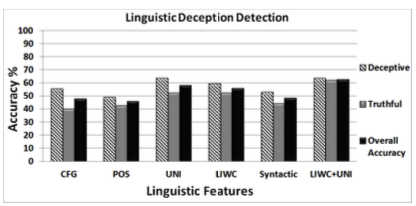
\includegraphics[width=7cm,keepaspectratio]{XX_Figures/Fig_Veronica_Linguistic.png}
	\caption{\footnotesize Accuracy obtenido por Aboulenien utilizando diferentes conjuntos de características linguisticas. \cite{Abouelenien2016AnalyzingApproach} .}
	\label{fig:Fig_Veronica_Linguistic}
\end{figure}

\begin{figure}[h!]
	\centering
	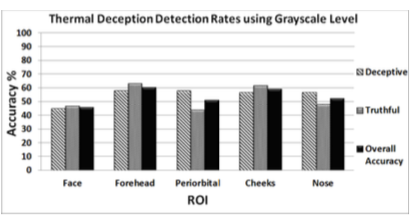
\includegraphics[width=7cm,keepaspectratio]{XX_Figures/Fig_Veronica_Termico_GS.png}
	\caption{\footnotesize Accuracy obtenido por Aboulenien utilizando características térmicas en escala de grises. \cite{Abouelenien2016AnalyzingApproach}.}
	\label{fig:Fig_Veronica_Termico_GS}
\end{figure}

\begin{figure}[h!]
	\centering
	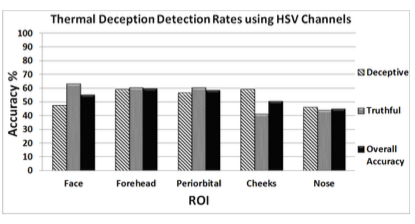
\includegraphics[width=7cm,keepaspectratio]{XX_Figures/Fig_Veronica_Termico_HSV.png}
	\caption{\footnotesize Accuracy obtenido por Aboulenien utilizando características térmicas en HSV. \cite{Abouelenien2016AnalyzingApproach}.}
	\label{fig:Fig_Veronica_Termico_HSV}
\end{figure}

En el año 2016, Verónica junto con un nuevo equipo creó un sistema  multimodal para detectar mentiras en la que integran características psicológicas, lingüísticas y térmicas basado en árboles de decisión, con el objetivo de crear un sistema completamente automático para detectar mentiras, de manera no invasiva y factible. En la Figura \ref{fig:Fig_Veronica_Linguistic}, se observan los resultados obtenidos a través de de 6 diferentes conjuntos de características, obteniendo una exactitud máximo de 62\% \cite{Abouelenien2016AnalyzingApproach}. Los resultados obtenidos extrayendo características térmicas en escala de grises se observan en la Figura \ref{fig:Fig_Veronica_Termico_GS} y en HSV en la Figura \ref{fig:Fig_Veronica_Termico_HSV}.\\

Krishnamurthy en el año 2018, creó un red neuronal multimodal capaz de detectar mentiras. Combinando características de video, audio, texto y micro-expresiones obtuvo hasta una exactitud del 96.14\%. Los diferentes modelos que utilizaron se muestran en la Figura \ref{fig:Figura_Navonil_Modelo}. De igual forma que Zhe Wu, realizaron las pruebas con individuos que pertenecen a un sistema nunca antes había visto (mismos sujetos no están en el conjunto de entrenamiento y conjunto de pruebas). Probaron el desempeño de su sistema por separado y con todas las modalidades. En la Tabla \ref{tab:Figura_Navonil_accuracy}, se puede observar que el modelo en el que solamente extraían características de los videos a través de una red 3D-CNN, obtenía una mayor exactitud que cualquier otro conjunto de características \cite{KrishnamurthyADetection}.\\

\begin{figure}[h!]
	\centering
	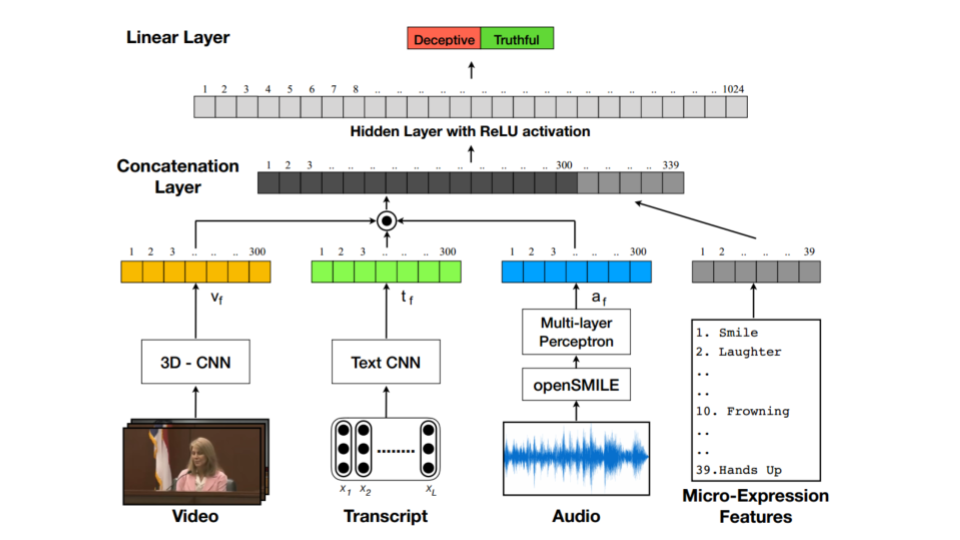
\includegraphics[width=13cm,keepaspectratio]{XX_Figures/Figura_Navonil_Modelo.png}
	\caption{\footnotesize Modelo de red neuronal multimodal utilizado por Krishnamurthy \cite{KrishnamurthyADetection}.}
	\label{fig:Figura_Navonil_Modelo}
\end{figure}

\begin{table}[h!]
\centering
    \begin{tabular}{|c|c|c|c|}
        \hline 
        Features & M LPu & MLPc & MLPh+c\tabularnewline
        \hline 
        \hline 
        Random & 43.90\% & 45.32\% & 48.51\%\tabularnewline
        \hline 
        Audio & 52.38\% & - & -\tabularnewline
        \hline 
        Visual & 93.08\% & - & -\tabularnewline
        \hline 
        Textutal (Static) & 80.16\% & - & -\tabularnewline
        \hline 
        Textual (Non-static) & 90.24\% & - & -\tabularnewline
        \hline 
        Micro-expressions & 76.16\% & - & -\tabularnewline
        \hline 
        All features (Static) & - & 90.49\% & 90.99\%\tabularnewline
        \hline 
        All features (Non\_static) & - & 95.24\% & 96.14\%\tabularnewline
        \hline 
    \end{tabular}
	\caption{\footnotesize Accuracy obtenido por Krishnamurthy con diferentes propuestas de modelos}
	\label{tab:Figura_Navonil_accuracy}
\end{table}

En este capítulo se presentaron varios estudios con diferentes propuestas no invasivas para detectar si una persona miente o no; estas propuestas obtienen mejores resultados para clasificar verdades y mentiras que el humano y algunos obtienen resultados similares al polígrafo. Vrij \cite{Vrij2000DetectingBehavior} a través de dos personas que extrajeron características manualmente en videos de personas mintiendo y diciendo verdades, anotando cuántas veces se desviaba la mirada, las veces que sonreía, movimientos de lo brazos y pies, etc, notaron que había diferencias en estas características entre las personas que decían mentiras y verdades, obteniendo una exactitud del 78\% para clasificar mentirosos y verdaderos. Verónica Pérez, una científica que ha trabajado en varios artículos que involucran la detección de mentiras junto con otros equipos, ha mostrado diferentes metodologías para clasificar verdades y mentiras de manera no invasiva. Además crearon un conjunto de datos que contienen personas mintiendo y diciendo verdades en juicios de Estados Unidos, el cual ha sido ocupado por algunos otros trabajos para detectar mentiras utilizando diferentes metodologías \cite{Perez-Rosas2015VerbalDetection,Abouelenien2016AnalyzingApproach}. Este conjunto de datos contiene a múltiples personas diciendo verdades y mentiras en la vida real, también se anotaron manualmente los gestos del rostro observados en los videos. A través de sistemas multimodales, combinando modalidades verbales y no verbales, Verónica y su equipo obtuvieron un 75\% de exactitud para clasificar verdades y mentiras en videos utilizando árboles de decisión. Después, con el uso de máquinas de soporte vectorial volvieron a probar un modelo multimodal pero utilizando dos conjuntos de datos, el que habían recopilado (`Trial') y uno nuevo que llamaron `Interview', ya que eran entrevistas hechas a diferentes personas en diferentes lugares. Ella y su equipo se dieron cuenta que cuando entrenaban su modelo con el conjunto de datos `Trial' y hacían las pruebas con el conjunto de datos `Interview' obtenían una exactitud del 58\% para clasificar los videos como verdad o mentira. A esta metodología de prueba se le llama Leave-one-person-out, la cuál esta basada en la validación cruzada leave-one-out con la diferencia que en lugar de dejar un conjunto de datos de prueba diferente al entrenamiento, se tienen personas diferentes en el conjunto de pruebas que en conjunto de entrenamiento. Utilizando la metodología Within-individual la cual se refiere a que en conjunto de pruebas y en el de entrenamiento se pueden encontrar las mismas personas, obtuvieron un 82\% para clasificar los datos del conjunto `Trial' y 79\% para el conjunto `Interview'. Krishnamurthy \cite{KrishnamurthyADetection} creando un sistema multimodal combinando información textual, visual, audio, microexpresiones manualmente anotadas y utilizando redes neuronales, fue capaz de clasificar videos como verdad o mentira con una exactitud del 96\% con la metodología de pruebas Leave-one-person-out en la que mencionan que las características que ayudaban a dar mejores resultados en el modelo multimodal eran las visuales las cuales fueron extraídas por una red convolucional 3D.
Otros trabajos se enfocaron en el uso de cámaras térmicas, tal es el caso de Abouelenien junto con Verónica \cite{Abouelenien2016AnalyzingApproach} en el cual crearon un sistema multimodal combinando el lenguaje no verbal, verbal y características térmicas convertidas a escala de grises y a HSV, obteniendo un 62\% de exactitud para clasificar verdades y mentiras. También Bashar \cite{Rajoub2014ThermalDetection} con el uso de cámaras térmicas y clasificación supervisada, logró clasificar verdades y mentiras con una exactitud del 58\% con la metodología Leave-one-person-out y 86\% con Within-individual utilizando árboles de decisión. Warmelink \cite{Warmelink2011ThermalAirports} construyó una herramienta computacional basada en la hipótesis en la que a través de imágenes térmicas, los mentirosos tienen una temperatura más alta que los verdaderos, obteniendo un 66\% para clasificar verdades y mentiras a través de respuestas fisiológicas medidas por cámaras térmicas.
En general se observa que diferentes trabajos han intentado solucionar el problema de detectar mentiras con métodos no invasivos y que deben existir características visuales que permiten a la computadora a través de diferentes extractores, instrumentos especiales, metodologías que involucran el movimiento del rostro, entre otros, obtener características importantes que permiten clasificar si una persona es deshonesto o es honesto en sus declaraciones. Esto motivó a que el presente trabajo se enfoque en el uso del lenguaje no verbal proporcionado por los fotogramas de un video y a utilizar aprendizaje profundo, ya que Krishnamurthy menciona tener mejores resultados para clasificar verdades y mentiras que las demás metodologías en el estado del arte utilizando aprendizaje profundo.

\begin{comment}
\ref{tab:ProblematicasPiloto}, se muestra una tabla de los diferentes métodos para detectar mentiras, la exactitud(accuracy) que tienen y las desventajas.

\begin{table}[h!]
\centering
    \begin{tabular}{|p{5cm}|p{2cm}|p{8cm}|}
        \hline 
        Método para detectar mentiras  & Accuracy  & Desventajas \tabularnewline
        \hline 
        \hline 
        Humanos no expertos & 54\%  & No conocen las pistas que delatan una mentira \tabularnewline
        \hline 
        Humanos expertos (Jueces, psicólogos, policias)  & 55\%  & Escenario interrogatorio, ver declaraciones varias veces, cada experto
        cree en diferentes pistas que delatan mentira, requieren de experiencia,
        high stake. \tabularnewline
        \hline 
        Polígrafo  & 70-95\%  & Ambiente controlado, calibración, horas para descifrar minutos, sistema
        invasivo, requiere de expertos, high stake. \tabularnewline
        \hline 
        Cámaras térmicas  & 64\%-87\%  & Ambiente controlado, calibración, costo elevado de material, high
        stake. \tabularnewline
        \hline 
        Lenguaje no verbal  & 60\%-96\%  & multimodales, algunos requieren de procesos manuales y requieren software
        especial. \tabularnewline
        \hline 
    \end{tabular}
    \caption{\footnotesize  Métodos para detectar mentiras.}.
    \label{tab:ProblematicasPiloto}
\end{table}
\end{comment}

\end{onehalfspacing}